\chapter{DOE - Teilfaktorielle Versuchspläne}
\label{sec: Hauptkapitel 4}

\section{Aufgabenstellung}
    In dieser Laboraufgabe soll die Frequenzlage eines Modes in Abhängigkeit von vier 
    zusätzlichen Massen untersucht werden. Die Eigenmoden des Flugzeugs ohne zusätzliche Massen 
    wurden bereits in Kapitel 2 bestimmt. Der Fokus dieses Versuchs liegt speziell auf dem 
    ersten Mode, der ohne Zusatzmassen  bei einer Frequenz von 5.048 [Hz] liegt.  
    \\

    \noindent
    Die Untersuchung soll anhand eines teilfaktoriellen Versuchsplans erfolgen.
    Dabei sollen verschiedene Kombinationen der Massen betrachtet werden, wobei 
    ausschließlich die Haupteffekte von Interesse sind.
%================================================================================

\section{Versuchsaufbau}
    Für den Versuch wird ein teilfaktorieller Versuchsplan mit vier Faktoren (Massen) 
    und zwei Stufen (-1 und +1) verwendet. Ziel ist es, den Einfluss der zusätzlichen Massen 
    auf die Frequenzlage des ersten Modes des Tragflügels zu bestimmen.  
    \\

    \noindent
    Da die gleichen Messgeräte wie in Kapitel \ref{sec: Hauptkapitel 1}
    verwendet werden, wird hier auf eine Auflistung verzichtet. Die verwendeten
    Messgeräte können in Tabelle \ref{tab: Geräteliste_EMA} nachgeschlagen
    werden.
    \\

    \noindent
    Da jeder Faktor zwei Stufen besitzt, würde ein vollständiger vollfaktorieller
    Versuchsplan insgesamt $2^4 = 16$ Kombinationen erfordern. Um die
    Versuchsanzahl zu reduzieren, wird ein teilfaktorieller Versuchsplan mit
    Auflösung IV verwendet. Dadurch müssen nur 8 Kombinationen untersucht werden.
    Diese Auflösung ist zur sicheren Bestimmung der Haupteffekte geeignet.
    \\

    \noindent
    Der Beschleunigungssensor bleibt während des gesamten Versuchs an einer festen Position 
    (Position \glqq 5 rot\grqq). Die genaue Anordnung der Sensor- und Massenpositionen ist in 
    Abbildung \ref{fig: Flieger_diskretisiert_2} dargestellt.

    % Bild - Diskretisiertes Modellflugzeug
    %--------------------------------------
    \begin{figure}[H]
        \centering
        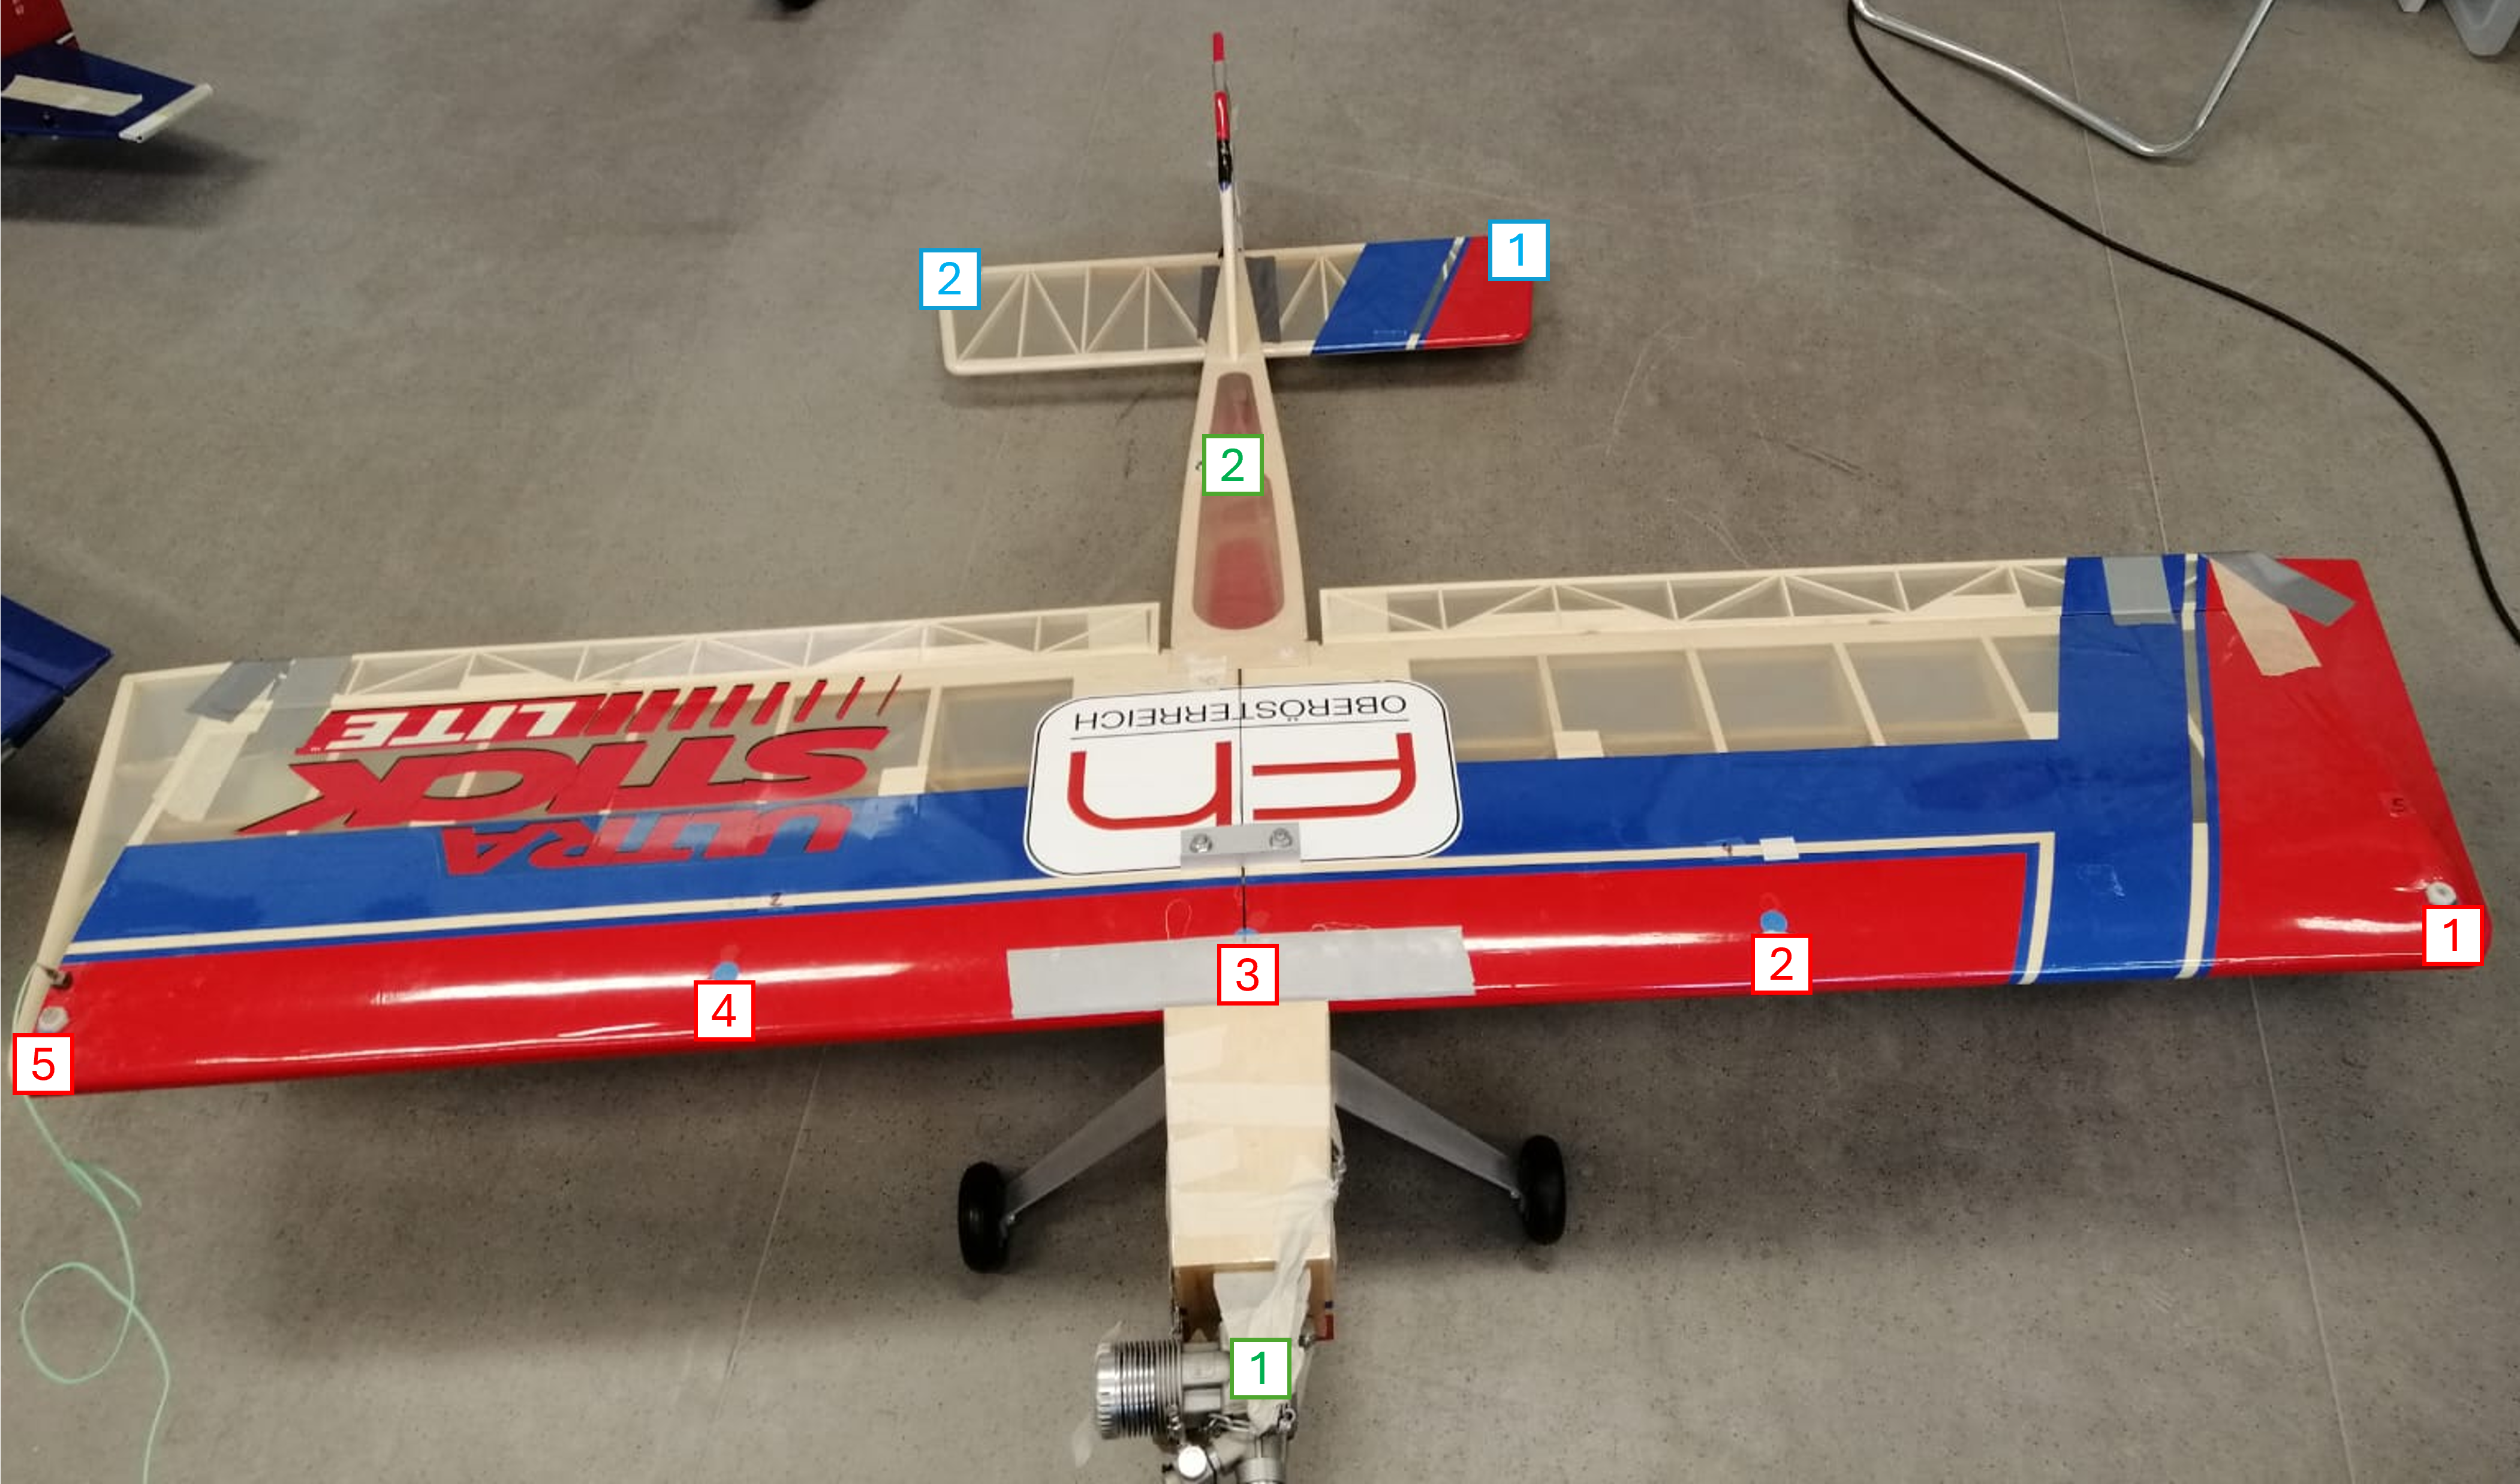
\includegraphics[width=0.95\textwidth]{Flieger_diskretisiert_Comp.png}
        \caption{Diskretisiertes Modellflugzeug mit Sensor- und Massenpositionen}
        \label{fig: Flieger_diskretisiert_2}
    \end{figure}

    \noindent
    Je nach getesteter Kombination werden die vier Massen an den vordefinierten
    Positionen des Tragflügels angebracht. Die Massen werden (bei Bedarf) an
    folgenden Positionen angebracht:

    \begin{itemize}
        \item Masse 1: Position \glqq 1 rot\grqq, 41 g  
        \item Masse 2: Position \glqq 5 rot\grqq, 44 g  
        \item Masse 3: Position \glqq 1 blau\grqq, 42 g  
        \item Masse 4: Position \glqq 2 blau\grqq, 44 g  
    \end{itemize}

    \noindent
    Für jede Kombination werden 3 Frequenzmessungen durchgeführt. Aus diesen
    Messungen wird anschließend der Mittelwert, die Standardabweichung sowie
    die Varianz berechnet.
    \newpage
%================================================================================
\section{Ergebnisse}
    Die Messergebnisse sind in Abbildung \ref{fig: Aufgabe4_Messungen} dargestellt.
    
    % Bild - Messergebnisse
    \begin{figure}[H]
        \centering
        \includegraphics[width=1\textwidth]{Aufgabe4_Messungen.png}
        \caption{Bestimmung der Modefrequenz aus drei Messungen}
        \label{fig: Aufgabe4_Messungen}
    \end{figure}
    
    \noindent
    Basierend auf den ermittelten Frequenzwerten und dem vorliegenden,
    teilfaktoriellen Versuchsplan wird eine Tabelle zur Berechnung der
    Haupteffekte sowie Wechselwirkungen zwischen den Massen erstellt
    (siehe Abbildung \ref{fig: Teilfaktorieller_Versuchsplan}).
    
    % Bild - Teilfaktorieller Versuchsplan
    \begin{figure}[H]
        \centering
        \includegraphics[width=1\textwidth]{Teilfaktorieller_Versuchsplan.png}
        \caption{Teilfaktorieller Versuchsplan mit berechneten Haupteffekten}
        \label{fig: Teilfaktorieller_Versuchsplan}
    \end{figure}
    
    \noindent
    Um die Signifikanz der einzelnen Effekte zu bestimmen, werden die
    Vertrauensquantile und somit das Signifikanzniveau ermittelt.
    Die grafische Darstellung der Signifikanzanalyse ist in Abbildung
    \ref{fig: Signifikanzniveau} zu sehen.
    
    % Bild - Signifikanzniveau
    \begin{figure}[H]
        \centering
        \includegraphics[width=0.95\textwidth]{Signifikanzniveau.png}
        \caption{Signifikanzanalyse der Haupteffekte und Wechselwirkungen}
        \label{fig: Signifikanzniveau}
    \end{figure}

    \noindent
    Die Signifikanzanalyse zeigt, dass alle Haupteffekte und Wechselwirkungen hoch signifikant sind, 
    mit Ausnahme des Faktors C, welcher Masse 3 entspricht. Die Position dieser
    Masse war hinten an der Finne des Flugzeugs (\glqq 1 blau\grqq). 
    Es ist auffällig, dass Masse 3 keinen Einfluss zeigt, während Masse 4
    (Faktor D) hoch signifikant ist. Da beide Massen annähernd gleich schwer sind
    und das Flugzeug weitgehend symmetrisch aufgebaut ist, wäre zu erwarten,
    dass entweder beide Massen (Masse 3 und 4) einen Einfluss haben oder
    keine der beiden.  